% document type and language
\documentclass[12pt]{article}

% standard packages
\usepackage{amsmath, bm, empheq, mathrsfs, natbib, cancel}

% normal margins
\usepackage[margin=1in]{geometry}

% plane blue hyperlinks
\usepackage[colorlinks]{hyperref}
\hypersetup{
	colorlinks = true,
	linkcolor=blue,
	citecolor=blue
}

% common macros
% Not sure where the following came from...maybe remove
\newcommand{\twochoices}[2]{\left\{ \begin{array}{lcc}
        \displaystyle #1 \\ \vspace{-10pt} \\
        \displaystyle #2 \end{array} \right. } %}

\newcommand{\threechoices}[3]{\left\{ \begin{array}{lcc}
        #1 \\ #2 \\ #3 \end{array} \right. }    %}

\newcommand{\fourchoices}[4]{\left\{ \begin{array}{lcc}
        #1 \\ #2 \\ #3 \\ #4 \end{array} \right. }      %}

\newcommand{\twovec}[2]{\left(\begin{array}{c} #1 \\ #2 \end{array}\right)}
\newcommand{\threevec}[3]{\left(\begin{array}{c} #1 \\ #2 \\ #3 \end{array}\right)}
\newcommand{\twomatrix}[4]{\left(\begin{array}{cc} #1 & #2 \\ #3 & #4 \end{array}\right)}

% MY MACROS

% MY EMAIL
\newcommand{\myemail}{loren.matilsky@gmail.com}

% MATH OPERATORS
\newcommand{\pderiv}[2]{\frac{\partial#1}{\partial#2}}
\newcommand{\matderiv}[1]{\frac{D#1}{Dt}}
\newcommand{\pderivline}[2]{\partial#1/\partial#2}
\newcommand{\parenfrac}[2]{\left(\frac{#1}{#2}\right)}
\newcommand{\brackfrac}[2]{\left[\frac{#1}{#2}\right]}
\newcommand{\bracefrac}[2]{\left\{\frac{#1}{#2}\right\}}
\newcommand{\av}[1]{\left\langle#1\right\rangle}
\newcommand{\avsph}[1]{\left\langle#1\right\rangle_{\rm{sph}}}
\newcommand{\avspht}[1]{\left\langle#1\right\rangle_{ {\rm sph}, t}}
\newcommand{\avt}[1]{\left\langle#1\right\rangle_{t}}
\newcommand{\avphi}[1]{\left\langle#1\right\rangle_{\phi}}
\newcommand{\avphit}[1]{\left\langle#1\right\rangle_{\phi,t}}
\newcommand{\avvol}[1]{\left\langle#1\right\rangle_{\rm{v}}}

\newcommand{\avalt}[1]{\langle#1\rangle}
\newcommand{\avaltsph}[1]{\langle#1\rangle_{\rm{sph}}}
\newcommand{\avaltt}[1]{\langle#1\rangle_{\rm{t}}}
\newcommand{\avaltphi}[1]{\langle#1\rangle_{\phi}}
\newcommand{\avaltphit}[1]{\langle#1\rangle_{\phi,t}}
\newcommand{\avaltvol}[1]{\langle#1\rangle_{\rm{v}}}

\newcommand{\sn}[2]{#1\times10^{#2}}
\newcommand{\define}{\coloneqq}
\newcommand{\definealt}{\equiv}
%\newcommand{\define}{\equiv}

% TEXT OPERATORS
\newcommand{\five}{\ \ \ \ \ }
\newcommand{\orr}{\text{or}\five }
\newcommand{\andd}{\text{and}\five }
\newcommand{\where}{\text{where}\five }
\newcommand{\with}{\text{with}\five }

% VECTOR SHORCUTS

% operators
\newcommand{\curl}{\nabla\times}
\newcommand{\Div}{\nabla\cdot}
\newcommand{\lap}{\nabla^2}
\newcommand{\dotgrad}{\cdot\nabla}
\newcommand{\ugrad}{\bm{u}\dotgrad}

% unit vectors
\newcommand{\e}{\hat{\bm{e}}}
\newcommand{\er}{\e_r}
\newcommand{\et}{\e_\theta}
\newcommand{\ep}{\e_\phi}
\newcommand{\el}{\e_\lambda}
\newcommand{\ez}{\e_z}
\newcommand{\exi}{\e_\xi}
\newcommand{\eeta}{\e_\eta}
\newcommand{\epol}{\e_{\rm{pol}}}

% REFERENCE STATE AND THERMO. VARIABLES
% may want to append this
\newcommand{\ofr}{(r)}

% reference-state constantsF_{\rm nr}
\newcommand{\cv}{c_{\rm{v}}}
\newcommand{\cp}{c_{\rm{p}}}
\newcommand{\cpcap}{C_{\rm{p}}}
\newcommand{\cvcap}{C_{\rm{v}}}
\newcommand{\cs}{c_{\rm s}}
\newcommand{\gasconst}{\mathcal{R}}
\newcommand{\gammaone}{\Gamma_1}
\newcommand{\omref}{\Omega_0}
\newcommand{\omrefvec}{\bm{\Omega}_0}

% total thermal variables (may wish to switch this stuff around later--I've always hated this notation of "no subscripts" = perturbation
\newcommand{\tot}{_{\rm{tot}}}
\newcommand{\rhotot}{\rho\tot}
\newcommand{\tmptot}{T\tot}
\newcommand{\prstot}{P\tot}
\newcommand{\stot}{S\tot}
\newcommand{\dsdrtot}{\frac{dS\tot}{dr}}
\newcommand{\dsdrtotline}{dS\tot/dr}

% reference or mean state
\newcommand{\rhoover}{\overline{\rho}}
\newcommand{\tmpover}{\overline{T}}
\newcommand{\prsover}{\overline{P}}
\newcommand{\entrover}{\overline{S}}
\newcommand{\inteover}{\overline{U}}
\newcommand{\enthover}{\overline{h}}
\newcommand{\heatover}{\overline{Q}}
\newcommand{\coolover}{\overline{C}}
\newcommand{\nsqover}{\overline{N^2}}
\newcommand{\gover}{\overline{g}}
\newcommand{\nuover}{\overline{\nu}}
\newcommand{\kappaover}{\overline{\kappa}}
\newcommand{\etaover}{\overline{\eta}}
\newcommand{\muover}{\overline{\mu}}
\newcommand{\deltaover}{\overline{\delta}}
\newcommand{\cpover}{\overline{\cpcap}}
\newcommand{\cvover}{\overline{\cvcap}}
\newcommand{\cssqover}{\overline{\cs^2}}

\newcommand{\rhotilde}{\tilde{\rho}}
\newcommand{\tmptilde}{\tilde{T}}
\newcommand{\prstilde}{\tilde{P}}
\newcommand{\entrtilde}{\tilde{S}}
\newcommand{\intetilde}{\tilde{U}}
\newcommand{\enthtilde}{\tilde{h}}
\newcommand{\heattilde}{\tilde{Q}}
\newcommand{\cooltilde}{\tilde{C}}
\newcommand{\nsqtilde}{\tilde{N^2}}
\newcommand{\gtilde}{\tilde{g}}
\newcommand{\nutilde}{\tilde{\nu}}
\newcommand{\kappatilde}{\tilde{\kappa}}
\newcommand{\etatilde}{\tilde{\eta}}
\newcommand{\mutilde}{\tilde{\mu}}
\newcommand{\deltatilde}{\tilde{\delta}}
\newcommand{\cptilde}{\tilde{\cpcap}}
\newcommand{\cvtilde}{\tilde{\cvcap}}
\newcommand{\cssqtilde}{\tilde{\cs^2}}

% perturbations from reference state
\newcommand{\rhoprime}{{\rho^\prime}}
\newcommand{\tmpprime}{{T^\prime}}
\newcommand{\prsprime}{{P^\prime}}
\newcommand{\entrprime}{{S^\prime}}
\newcommand{\inteprime}{{U^\prime}}
\newcommand{\enthprime}{{h^\prime}}

\newcommand{\rhohat}{\hat{\rho}}
\newcommand{\tmphat}{\hat{T}}
\newcommand{\prshat}{\hat{P}}
\newcommand{\entrhat}{\hat{S}}
\newcommand{\intehat}{\hat{U}}
\newcommand{\enthhat}{\hat{h}}

\newcommand{\rhoone}{\rho_1}
\newcommand{\tmpone}{T_1}
\newcommand{\prsone}{P_1}
\newcommand{\entrone}{S_1}
\newcommand{\inteone}{U_1}
\newcommand{\enthone}{h_1}

\newcommand{\pomega}{\varpi}

\newcommand{\fluxnr}{F_{\rm nr}}
\newcommand{\fluxnrtilde}{\widetilde{F_{\rm nr}}}

\newcommand{\grav}{g}
\newcommand{\vecg}{\bm{g}}
\newcommand{\geff}{g_{\rm{eff}}}
\newcommand{\vecgeff}{\bm{g}_{\rm{eff}}}

\newcommand{\heat}{Q}
\newcommand{\buoyfreq}{N}
\newcommand{\nsq}{N^2}

% reference-state derivatives
\newcommand{\dlnrho}{\frac{d\ln\rhoover}{dr}}
\newcommand{\dlntmp}{\frac{d\ln\tmpover}{dr}}
\newcommand{\dlnprs}{\frac{d\ln\prsover}{dr}}
\newcommand{\dsdr}{\frac{d\overline{S}}{dr}}

\newcommand{\dlnrholine}{d\ln\rhoover/dr}
\newcommand{\dlntmpline}{d\ln\tmpover/dr}
\newcommand{\dlnprsline}{d\ln\prsover/dr}
\newcommand{\dsdrline}{d\overline{S}/dr}

\newcommand{\hrho}{H_\rho}
\newcommand{\hprs}{H_{\rm{p}}}

% FLUID VARIABLES

% vector fields
\newcommand{\vecu}{\bm{u}}
\newcommand{\vecb}{\bm{B}}
\newcommand{\vecom}{\bm{\omega}}
\newcommand{\vecj}{\bm{\mathcal{J}}}

\newcommand{\upol}{\vecu_{\rm{pol}}}
\newcommand{\bpol}{\vecb_{\rm{pol}}}

\newcommand{\urad}{u_r}
\newcommand{\ut}{u_\theta}
\newcommand{\up}{u_\phi}
\newcommand{\ul}{u_\lambda}
\newcommand{\uz}{u_z}

\newcommand{\omr}{\omega_r}
\newcommand{\omt}{\omega_\theta}
\newcommand{\omp}{\omega_\phi}
\newcommand{\oml}{\omega_\lambda}
\newcommand{\omz}{\omega_z}

\newcommand{\br}{B_r}
\newcommand{\bt}{B_\theta}
\newcommand{\bp}{B_\phi}
\newcommand{\bl}{B_\lambda}
\newcommand{\bz}{B_z}

\newcommand{\jr}{\mathcal{J}_r}
\newcommand{\jt}{\mathcal{J}_\theta}
\newcommand{\jp}{\mathcal{J}_\phi}
\newcommand{\jl}{\mathcal{J}_\lambda}
\newcommand{\jz}{\mathcal{J}_z}

% spherical coordinates
\newcommand{\cost}{\cos\theta}
\newcommand{\sint}{\sin\theta}
\newcommand{\cott}{\cot\theta}
\newcommand{\rsint}{r\sint}
\newcommand{\orsint}{\frac{1}{\rsint}}
\newcommand{\orsintline}{(1/\rsint)}
\newcommand{\rt}{r\theta}


% SIMULATION GEOMETRY
%s subscripts
\newcommand{\minn}{_{\rm{min}}}
\newcommand{\maxx}{_{\rm{max}}}
\newcommand{\inn}{_{\rm{in}}}
\newcommand{\out}{_{\rm{out}}}
\newcommand{\bott}{_{\rm{bot}}}
\newcommand{\midd}{_{\rm{mid}}}
\newcommand{\topp}{_{\rm{top}}}
\newcommand{\bcz}{_{\rm{bcz}}}
\newcommand{\ov}{_{\rm{ov}}}
\newcommand{\rms}{_{\rm{rms}}}
\newcommand{\const}{_{\rm{const}}}

\newcommand{\lmax}{{\ell_{\rm{max}}}}

% SOLAR AND STELLAR VARIABLES
\newcommand{\rsun}{R_\odot}
\newcommand{\rtach}{r_t}
\newcommand{\lsun}{L_\odot}
\newcommand{\omsun}{\Omega_\odot}

\newcommand{\msun}{M_\odot}
\newcommand{\rstar}{R_*}
\newcommand{\lstar}{L_*}
\newcommand{\mstar}{M_*}
\newcommand{\omstar}{\Omega_*}

\newcommand{\rearth}{R_\oplus}
\newcommand{\omearth}{\Omega_\oplus}
\newcommand{\mearth}{M_\oplus}

% TORQUE DEFINITIONS
\newcommand{\taurs}{\tau_{\rm{rs}}}
\newcommand{\taurad}{\tau_{\rm{rad}}}
\newcommand{\taums}{\tau_{\rm{ms}}}
\newcommand{\taumm}{\tau_{\rm{mm}}}
\newcommand{\taumc}{\tau_{\rm{mc}}}
\newcommand{\tauv}{\tau_{\rm{v}}}
\newcommand{\taumag}{\tau_{\rm{mag}}}

% stellar time scales
\newcommand{\pes}{{P_{\rm{ES}}}}
\newcommand{\pessun}{{P_{ {\rm ES}, \odot}}}
\newcommand{\pnu}{{P_{\nu}}}
\newcommand{\pkappa}{{P_{\kappa}}}
\newcommand{\peta}{{P_{\eta}}}
\newcommand{\prot}{{P_{\rm{rot}}}}
\newcommand{\pequil}{{P_{\rm{eq}}}}
\newcommand{\tequil}{{t_{\rm{eq}}}}
\newcommand{\tmax}{{t_{\rm{max}}}}
\newcommand{\pcyc}{{P_{\rm{cyc}}}}
\newcommand{\omcyc}{{\omega_{\rm{cyc}}}}
\newcommand{\pcycm}{{P_{{\rm cyc}, m}}}
\newcommand{\omcycm}{{\omega_{{\rm{cyc}}, m}}}
% NON-DIMENSIONAL NUMBERS

% input non-d
\newcommand{\nrho}{N_\rho}

\newcommand{\ra}{{\rm{Ra}}}
\newcommand{\ramod}{\ra^*}
\newcommand{\raf}{\ra_{\rm{F}}}
\newcommand{\rafmod}{\raf^*}

\newcommand{\pr}{{\rm{Pr}}}
\newcommand{\prm}{{\rm{Pr_m}}}

\newcommand{\di}{{\rm{Di}}}

\newcommand{\ek}{{\rm{Ek}}}
\newcommand{\ta}{{\rm{Ta}}}

%\newcommand{\he}{{\rm{He}}}

\newcommand{\bu}{{\rm{Bu}}}
\newcommand{\bumod}{{\rm{Bu^*}}}
\newcommand{\bvisc}{{\rm{Bu_{visc}}}}
\newcommand{\brot}{{\rm{Bu_{rot}}}}

% output non-d
\newcommand{\ro}{{\rm{Ro}}}
\newcommand{\lo}{{\rm{Lo}}}
\newcommand{\roc}{{\rm{Ro_c}}}

\newcommand{\re}{{\rm{Re}}}
\newcommand{\rem}{{\rm{Re_m}}}

% FLUX ALIASES
\newcommand{\flux}{{\bm{\mathcal{F}}}}
\newcommand{\fcond}{\flux_{\rm{cond}}}
\newcommand{\frad}{\flux_{\rm{rad}}}
\newcommand{\fluxscalar}{{\mathcal{F}}}
\newcommand{\fcondscalar}{\fluxscalar_{\rm{cond}}}
\newcommand{\fenthscalar}{\fluxscalar_{\rm{enth}}}

% UNITS
\newcommand{\gram}{{\rm{g}}}
\newcommand{\cm}{{\rm{cm}}}
\newcommand{\second}{{\rm{s}}}
\newcommand{\gauss}{{\rm{G}}}
\newcommand{\kelv}{{\rm{K}}}
\newcommand{\unitent}{{\rm{erg\ g^{-1}\ K^{-1}}}}
\newcommand{\uniten}{\rm{erg}\ \cm^{-3}}
\newcommand{\unitprs}{\rm{dyn}\ \cm^{-2}}
\newcommand{\unitrho}{\gram\ \cm^{-3}}
\newcommand{\stoke}{\rm{cm^2\ s^{-1}}}

% MEAN FIELD THEORY
\newcommand{\meanb}{\overline{\bm{B}}}
\newcommand{\flucb}{\bm{B}^\prime}
\newcommand{\totb}{\bm{B}}

\newcommand{\meanv}{\overline{\bm{v}}}
\newcommand{\flucv}{\bm{v}^\prime}
\newcommand{\totv}{\bm{v}}

\newcommand{\emf}{\bm{\mathcal{E}}}
\newcommand{\meanemf}{\overline{\bm{\mathcal{E}}}}
\newcommand{\meanbpol}{\overline{\bm{B}_{\rm{pol}}}}

% SIMULATION CODES
\newcommand{\rayleigh}{\texttt{Rayleigh}}
\newcommand{\rayleigha}{\texttt{Rayleigh 0.9.1}}
\newcommand{\rayleighb}{\texttt{Rayleigh 1.0.1}}

\newcommand{\eulag}{\texttt{EULAG}}
\newcommand{\eulagmhd}{\texttt{EULAG-MHD}}
\newcommand{\ash}{\texttt{ASH}}
\newcommand{\rsst}{\texttt{RSST}}
\newcommand{\rtdt}{\texttt{R2D2}}
\newcommand{\pencil}{\texttt{Pencil}}

% other macros
\newcommand{\vecrot}{\bm{\Omega}}
\newcommand{\vecr}{\bm{r}}
\newcommand{\xpar}{x_\parallel}
\newcommand{\epar}{\e_\parallel}
\newcommand{\upar}{u_\parallel}
\newcommand{\uperp}{\vecu_\perp}
\newcommand{\veci}{\bm{I}}

% date, author, title
\date{\today}
\author{Loren Matilsky}
\title{Induction term in spherical coordinates}

\begin{document}
\maketitle

\section{The problem with the traditional induction terms}
We consider the ideal (resistance-free) magnetohydrodynamic (MHD) induction equation:
\begin{align}
	\five\pderiv{\vecb}{t} &= \curl(\vecu\times\vecb) \label{eq:ind1}\define\veci,\\
	&= \vecb\dotgrad\vecu - \vecu\dotgrad\vecb -(\Div\vecu)\vecb, \label{eq:ind2}
\end{align}
where $\vecb$ and $\vecu$ are the vector magnetic and velocity fields (respectively) and $\veci$ is the vector induction. The three terms on the right-hand-side of Equation \eqref{eq:ind2} are often interpreted as ``shear," ``advection," and ``compression," respectively. However, this interpretation is problematic in general for two reasons:

\begin{enumerate}
	\item The so-called shear and compression terms contain sub-terms that cancel; in particular, only velocity motions \textit{transverse} to magnetic-field lines can shear or compress. \label{enum:problem1}
	\item Solid-body rotation (which is a non-shearing motion that simply rotates the whole field configuration) shows up in the so-called shear and advection terms in a strange way. \label{enum:problem2}
\end{enumerate}

Finally, even after these issues have been addressed, resolving the final terms into a particular curvilinear system (e.g., spherical coordinates) seems to present a major headache. Our goal here is to explain fully how these problems emerge and propose a tentative solution for the case of spherical coordinates. 

\section{Transverse shear and compression}
To see how Problem \ref{enum:problem1} arises, we decompose the velocity field into components parallel and perpendicular to the local direction of $\vecb$:
\begin{align}
	\vecu &\define \upar\epar + \uperp
\end{align} 
Obviously $\vecb=B\xpar$, where $B=|\vecb|$. We denote the Cartesian distance along $\vecb$ by $\xpar$. We also decompose $\vecu$ into its parallel and perpendicular components:
\begin{align}
	\Div\vecu=\pderiv{\upar}{\xpar}+\nabla_\perp\cdot\uperp
\end{align}
We then calculate
\begin{align}
	\vecb\dotgrad\vecu - (\Div\vecu)\vecb&=B\pderiv{}{\xpar}(\upar\epar + \uperp) -\left(\pderiv{\upar}{\xpar}+\nabla_\perp\cdot\uperp\right)B\epar\nonumber\\
	&= \cancel{B\pderiv{\upar}{\xpar}\epar} + B\pderiv{\uperp}{\xpar} -\cancel{\pderiv{\upar}{\xpar} B\epar} - (\nabla_\perp\cdot\uperp)B\epar\nonumber\\
	&= \vecb\dotgrad\uperp - (\nabla_\perp\cdot\uperp)\vecb.
\end{align}
Thus, only motions transverse to the local field line (i.e., $\uperp$) can shear or compress $\vecb$.  

\section{Rigid rotation}
To see how Problem \ref{enum:problem2} arises, we consider a velocity field due to rigid rotation at constant angular velocity $\Omega$ about the $z$-axis in a cylindrical coordinate system:
\begin{subequations}
	\begin{align}
		\vecrot &= \Omega\ez=\text{constant}\\
		\vecu&=\vecrot\times\bm{r} = \Omega\lambda\ep
	\end{align}
\end{subequations}
Here, $\lambda$ is the cylindrical radius, $\phi$ the longitude, and $z$ the axial coordinate. In general,  $\e_{(\cdots)}$ denotes a unit vector in the direction of its subscript. We calculate:
\begin{align}
	\Div\vecu&=\Div(\vecrot\times\bm{r})\nonumber\\
	&= \vecrot\dotgrad\times\vecr-\vecr\dotgrad\times\vecrot\nonumber\\
	&= 0\five\text{no compression for rigid rotation (obviously).}
\end{align}
Then:
\begin{align}
	\vecb\dotgrad\vecu&=(\vecb\dotgrad)(\vecrot\times\vecr)\nonumber\nonumber\\
	&= \vecrot\times[(\vecb\dotgrad)(\vecr)]\\
	&= \vecrot\times\vecb\five\text{``shear" for rigid rotation}.
\end{align}
Finally:
\begin{align*}
	-\vecu\dotgrad\vecb &= -\Omega\lambda\ep\dotgrad\vecb\\
	&=-\Omega\pderiv{}{\phi}(B_\lambda\el+B_\phi\ep+B_z\ez)\\
	&=-\Omega\sum_\alpha\left(\pderiv{B_\alpha}{\phi}\right)\e_\alpha-\Omega\sum_\alpha B_\alpha\pderiv{\e_\alpha}{\phi},
\end{align*}
where the index $\alpha$ runs over the three cylindrical coordinates. Note that in the cylindrical coordinate system (or indeed any coordinate system with an axis of rotational symmetry), $\pderivline{\e_\alpha}{\phi}=\e_z\times\e_\alpha$ for each $\alpha$. Thus,
\begin{align*}
	-\Omega\sum_\alpha B_\alpha\pderiv{\e_\alpha}{\phi} &= -\Omega\sum_\alpha B_\alpha\ez\times\e_\alpha\\
	&=-\Omega\ez\times\sum_\alpha B_\alpha\e_\alpha\\
	&=-\vecrot\times\vecb
\end{align*}
and so
\begin{align}
	-\vecu\dotgrad\vecb &= -\Omega\sum_\alpha\left(\pderiv{B_\alpha}{\phi}\right)\e_\alpha-\vecrot\times\vecb \five \text{``advection" for rigid rotation}.
\end{align}
Mathematically, in any coordinate system with a $z$-axis of rotational symmetry, the action of rigid rotation is as follows:
\begin{subequations}
\begin{align}
	\pderiv{\vecb}{t}&=\curl[(\vecrot\times\vecr)\times\vecb]\nonumber\\
	&= \sum_\alpha\left(-\Omega\pderiv{B_\alpha}{\phi}\right)\e_\alpha \label{eq:rottransport1}\\
	\orr \left(\pderiv{}{t}+\Omega\pderiv{}{\phi}\right)B_\alpha&=0\five\text{for each $\alpha$}.\label{eq:rottransport2}
\end{align}
\end{subequations}
If you think about it, this makes sense: All the rigid rotation does is rotate the whole field configuration around the $z$-axis at the rate $\Omega$. If you decide to also rotate at $\Omega$ (so your personal Eulerian time derivative is $\pderivline{}{t}+\Omega\pderivline{}{\phi}$), then each component of the magnetic-field configuration should remain the same in your frame. Note that rotation does \textit{not} advect the vector magnetic field (like the term $-\vecu\dotgrad\vecb$ viewed on its own would suggest), but rather advects the field \textit{components} (as if they were scalars) in any coordinate system with an axis of rotational symmetry. 

\section{Solution for spherical coordinates}
Resolving these issues fully for the spherical coordinate system seems complicated and I am not fully sure how to do it! In particular (for ``full" resolution) we should, separately at each point ($r$,$\theta$,$\phi$):
\begin{enumerate}
	\item Form a local Cartesian coordinate system, say ($x_1$, $x_2$, $x_3$), whose origin lies at the point $(r,\theta,\phi)$. At the origin, ($\e_1$, $\e_2$, $\e_3$) will coincide with ($\er$, $\et$, $\ep$). But slightly away from the origin, ($\e_1$, $\e_2$, $\e_3$) will stay fixed while ($\er$, $\et$, $\ep$) curve away. 
	\item Calculate the velocity-gradient tensor: $\pderivline{u_1}{x_1},\pderivline{u_2}{x_1}, \pderivline{u_3}{x_1}$, etc. While calculating derivatives, be careful to differentiate along the Cartesian coordinates, \textit{not} the curvilinear ones or along the actual $\vecb$-line). Express the final tensor components in spherical coordinates.
	\item Rotate ``into $\vecb$" to form a new primed coordinate system (such that $\e_1^\prime$ points along $\vecb$), calculate the $\pderivline{u_j^\prime}{x_i^\prime}$, and thus form $\pderivline{\upar}{\xpar}$ and $\pderivline{\uperp}{\xpar}$ (note that $\nabla_\perp\cdot\uperp=\Div\vecu- \pderivline{\upar}{\xpar}$). Note that the direction cosines $\e_1^\prime$ makes with ($\e_1$, $\e_2$, $\e_3$) are simply $\br/|\vecb|, \bt/|\vecb|, \bp/|\vecb|$, respectively. Note that both unit vectors and vector components transform like $x_1^\prime=\sum_{j=1}^3R_{1j}x_j$, where $R_{1j}$ is the $j^{th}$ direction cosine.  
	\item Subtract the part of $\uperp$ corresponding to solid-body rotation and put it in the form of Equation \eqref{eq:rottransport1}. 
	\item Exult, because I haven't been able to do this!
\end{enumerate}
Instead of addressing the full problem as just described, I have brute-forced my way into a quasi-solution, canceling obvious terms and expressing what seem to be ``transverse shear with no solid-body rotation," ``transverse compression," and advection. 

We write:
\begin{align*}
	I_r =\ &\cancel{  \br\pderiv{\ur}{r}  }    +    \frac{\bt}{r}\pderiv{\ur}{\theta}    +    \frac{\bp}{\rsint}\pderiv{\ur}{\phi}    -    \bcancel{   \frac{\bt\ut+\bp\up}{r}  }
	\\
	&-\ugrad\br    +    \bcancel{   \frac{\ut\bt+\up\bp}{r}  }
	\\
	&- \left[   \cancel{\pderiv{\ur}{r}}    +     \frac{2\ur}{r}    +    \frac{1}{r}\left(  \pderiv{\ut}{\theta}    +   \cott\ut  \right)    +    \orsint\pderiv{\up}{\phi}   \right] \br
\end{align*}
or
\begin{subequations}\label{eq:indr}
\begin{alignat}{2}
	I_r = \  &  \left(   \frac{\bt}{r}\pderiv{}{\theta}    +    \frac{\bp}{\rsint}\pderiv{}{\phi}   \right) \ur &&  \five \text{$r$: transverse shear}
	\\
	&-\ \ugrad\br && \five\text{$r$: advection}
	\\
	  &-\left( \frac{1}{r} \pderiv{\ut}{\theta}    +    \orsint \pderiv{\up}{\phi}    +    \frac{2\ur}{r}    +     \frac{\cott\ut}{r}  \right)  \br   && \five \text{$r$: transverse compression}
\end{alignat}
\end{subequations}

Then, for $I_\theta$:
\begin{align*}
	I_\theta = & \br\pderiv{\ut}{r}      +  \cancel{  \frac{\bt}{r}\pderiv{\ut}{\theta}  }    +    \frac{\bp}{\rsint}\pderiv{\ut}{\phi}    +     \frac{\bt\ur}{r}    -    \bcancel{  \frac{\cott\bp\up}{r}  }
	\\
	&-\ugrad\bt    -    \frac{\ut\br}{r}    +    \bcancel{  \frac{\cott\up\bp}{r}  }
	\\
	&- \left[   \pderiv{\ur}{r}    +     \frac{2\ur}{r}    +    \frac{1}{r}\left(  \cancel{ \pderiv{\ut}{\theta} }    +   \cott\ut  \right)    +    \orsint\pderiv{\up}{\phi}   \right] \bt
\end{align*}
or
\begin{subequations}\label{eq:indt}
	\begin{alignat}{2}
		I_\theta = \  &  r \left(   \br\pderiv{}{r}    +    \frac{\bp}{\rsint}\pderiv{}{\phi}   \right)  \left(  \frac{\ut}{r}  \right) &&  \five \text{$\theta$: transverse shear}
		\\
		&-\ \ugrad\bt && \five\text{$\theta$: advection}
		\\
		&-\left(  \pderiv{\ur}{r}    +     \orsint \pderiv{\up}{\phi}    +    \frac{\ur}{r}    +    \frac{\cott\ut}{r}  \right) \bt   && \five \text{$\theta$: transverse compression}
	\end{alignat}
\end{subequations}

Finally, for $I_\phi$:
\begin{align*}
	I_\phi = & \br\pderiv{\up}{r}      +   \frac{\bt}{r}\pderiv{\up}{\theta}    +    \cancel{  \frac{\bp}{\rsint}\pderiv{\up}{\phi}  }    +     \frac{\bp\ur}{r}    +    \bcancel{  \frac{\cott\bp\ut}{r}   }
	\\
	&-\ugrad\bp    -       \frac{\up\br}{r}    -    \frac{\cott\up\bt}{r} 
	\\
	&- \left[   \pderiv{\ur}{r}    +     \frac{2\ur}{r}    +    \frac{1}{r}\left(  \pderiv{\ut}{\theta}     +   \bcancel{  \cott\ut  }  \right)    +    \cancel{  \orsint\pderiv{\up}{\phi}  }   \right] \bp
\end{align*}
or
\begin{subequations}\label{eq:indp}
	\begin{alignat}{2}
		I_\phi = \  &  \rsint \left(   \br\pderiv{}{r}    +    \frac{\bt}{r}\pderiv{}{\theta}   \right)  \left(  \frac{\up}{\rsint}  \right) &&  \five \text{$\phi$: transverse shear}
		\\
		&-\ \ugrad\bp && \five\text{$\phi$: advection}
		\\
		&-\left(  \pderiv{\ur}{r}    +     \frac{1}{r} \pderiv{\ut}{\theta}    +    \frac{\ur}{r}     \right) \bp   && \five \text{$\phi$: transverse compression}
	\end{alignat}
\end{subequations}

\section{Transverse compression}
Here we show that the ``transverse compression" terms defined in Equations \eqref{eq:indr}--\eqref{eq:indp} make sense. The key point is that we must be careful (in calculating $\nabla_\perp\cdot\uperp$) when differentiating along $\theta$ or $\phi$, because the local spherical unit vectors will all be changing. For example the divergence ``transverse to $\er$" is not simply $\Div(\ut\et + \up\ep)$; there are also curvature terms. 

  \begin{figure}
	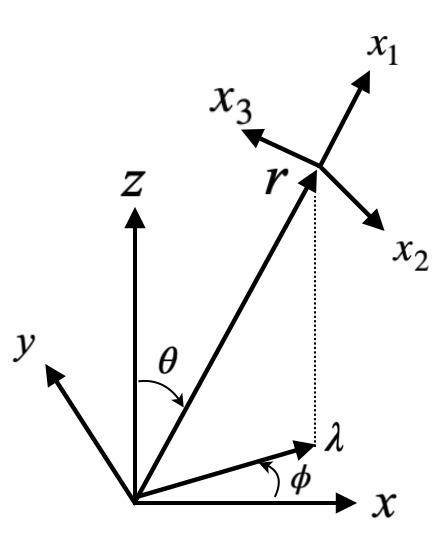
\includegraphics[scale=0.4]{Fig1_coordinate_systems.png}\hfill 	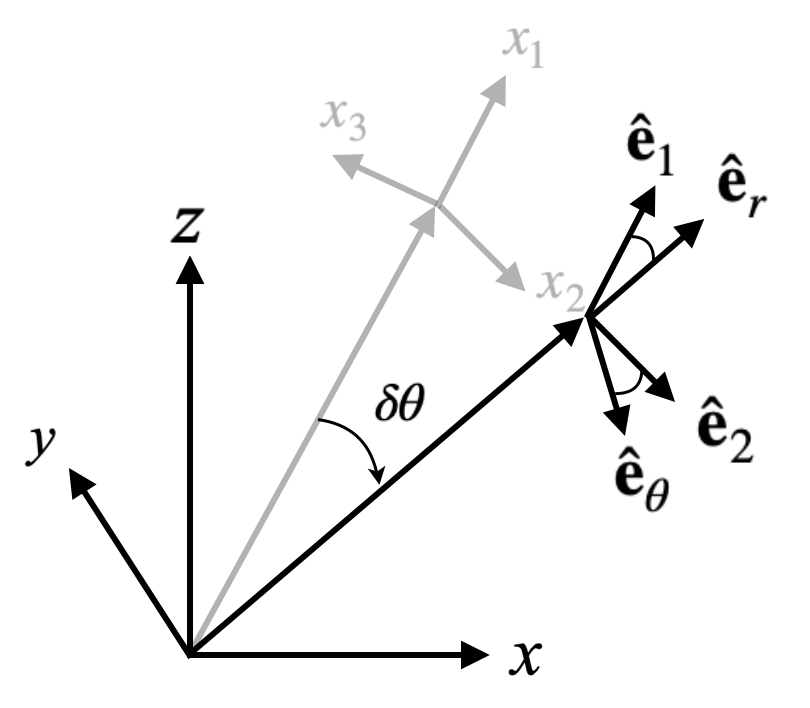
\includegraphics[scale=0.35]{Fig2_Pertx2.png}
	\caption{\textit{Left}: Schematic of coordinate systems used here, their relation to one another, and each coordinate's meaning. Note that $(x,y,z) = (\lambda\cos\phi, \lambda\sin\phi, z) = (\rsint\cos\phi, \rsint\sin\phi, r\cost)$. The local Cartesian system $(x_1,x_2,x_3)$ has its origin at the point $(r,\theta,\phi)$, where $(\e_1,\e_2,\e_3) = (\er, \et, \ep)$. \textit{Right}: Away from the origin, the unit vectors no longer coincide. We show the relationship between the spherical-coordinate unit vectors and the Cartesian unit vectors when $\theta\rightarrow\theta+\delta\theta$ (or equivalently, $x_2=0\rightarrow  \delta x_2$). }
	\label{fig:coords}
\end{figure}

Figure \ref{fig:coords} shows schematically how this works. We set up a local Cartesian coordinate system (with origin at the point $(r,\theta,\phi)$) denoted by $(x_1,x_2,x_3)$. As we differentiate $\vecu$, the spherical-coordinate unit vectors change, while the Cartesian ones stay fixed. In particular, if we move from $(r,\theta,\phi)\rightarrow (r+\delta r, \theta + \delta\theta, \phi + \delta\phi)$ (or equivalently in the Cartesian system, $(0, 0, 0)\rightarrow (\delta x_1, \delta x_2, \delta x_3)$), we find the following (to first order in the $\delta$'s):
\begin{subequations}
\begin{align}
	u_1 &= \ur - (\delta\theta)\ut - (\sint\delta\phi)\up,\\ 
	u_2 &= \ut + (\delta\theta)\ur - (\cost\delta\phi)\up, \\ 
	\andd u_3 &= \up + (\sint\delta\phi)\ur + (\cost\delta\phi)\ut.
\end{align}
\end{subequations}
And trivially:
\begin{subequations}
	\begin{align}
		\delta x_1 &= \delta r \\ 
		\delta x_2 &= r\delta\theta\\
		\delta x_3 &= \rsint\delta\phi
	\end{align}
\end{subequations}
We thus compute:
\begin{align}
	\pderiv{u_1}{x_1} &= \lim_{\delta x_1\rightarrow0}\frac{u_1(\delta x_1, 0, 0) - u_1(0,0,0)}{\delta x_1}\nonumber\\
	&=  \lim_{\delta r\rightarrow0}\frac{\ur(r+\delta r, \theta, \phi) - \ur(r,\theta,\phi)}{\delta r}\nonumber\\
	&= \pderiv{\ur}{r}
\end{align}
That was the easy one! Now for the curvy ones:
\begin{align}
	\pderiv{u_2}{x_2} &= \lim_{\delta x_2\rightarrow0}\frac{u_2(0, \delta x_2, 0) - u_2(0,0,0)}{\delta x_2}\nonumber\\
	&=  \lim_{\delta \theta\rightarrow0}\frac{\ut(r, \theta+\delta\theta, \phi) + \ur(r,\theta+\delta\theta,\phi)\delta\theta - \ut(r,\theta,\phi)}{r\delta\theta}\nonumber\\
	&= \lim_{\delta \theta\rightarrow0}\frac{\ut(r, \theta+\delta\theta, \phi) - \ut(r,\theta,\phi)}{r\delta\theta} + \lim_{\delta \theta\rightarrow0} \frac{\ur(r,\theta+\delta\theta,\phi)}{r} \nonumber\\
	&= \frac{1}{r}\pderiv{\ut}{\theta} + \frac{\ur}{r}
\end{align}
And finally:
\begin{align}
	\pderiv{u_3}{x_3} &= \lim_{\delta x_3\rightarrow0}\frac{u_3(0,0,  \delta x_3) - u_3(0,0,0)}{\delta x_3}\nonumber\\
	&=  \lim_{\delta \phi\rightarrow0}  \frac{\up(r, \theta, \phi+\delta\phi) + (\sint\ur + \cost\ut)\delta\phi - \up(r,\theta,\phi) } {\rsint\delta\phi}\nonumber\\
	&= \orsint\pderiv{\up}{\phi} + \frac{\ur}{r} + \frac{\cott\ut}{r}
\end{align}
We thus find the various components of transverse divergence: 
\begin{align}
	(\Div\vecu)_{\perp\ \text{to}\ r} &= \pderiv{u_2}{x_2} + \pderiv{u_3}{x_3} \nonumber\\
	&= \frac{1}{r} \pderiv{\ut}{\theta}    +    \orsint \pderiv{\up}{\phi}    +    \frac{2\ur}{r}    +     \frac{\cott\ut}{r},\\
	(\Div\vecu)_{\perp\ \text{to}\ \theta} &= \pderiv{u_1}{x_1} + \pderiv{u_3}{x_3} \nonumber\\
	&=  \pderiv{\ur}{r}    +     \orsint \pderiv{\up}{\phi}    +    \frac{\ur}{r}    +    \frac{\cott\ut}{r} 
	\andd 	(\Div\vecu)_{\perp\ \text{to}\ \phi} &= \pderiv{u_1}{x_1} + \pderiv{u_2}{x_2} \nonumber\\	
	 &= \pderiv{\ur}{r}    +     \frac{1}{r} \pderiv{\ut}{\theta}    +    \frac{\ur}{r} 
\end{align}
\end{document}